\documentclass[12pt, letterpaper]{book}

% Standard LaTeX Packages
\usepackage[utf8]{inputenc}
\usepackage[T1]{fontenc}
\usepackage{lmodern} % For better font quality
\usepackage{amsmath}
\usepackage{amssymb}
\usepackage{mathtools}
\usepackage{graphicx}
\usepackage{tikz} % Keep if diagrams are still needed
\usepackage{booktabs} % For professional quality tables
\usepackage{multicol} % If multicolumn layouts are still desired in some parts
\usepackage{xcolor} % For color definitions, if still needed
\usepackage{geometry} % For page layout
\usepackage{fancyhdr} % For custom headers and footers
\usepackage{hyperref} % For clickable links (TOC, references)

% Page geometry
\geometry{
    letterpaper,
    top=1in,
    bottom=1in,
    left=1.25in,
    right=1.25in,
    headheight=15pt
}

% Color definitions (if needed, or can be removed/modified)
\definecolor{mDarkTeal}{HTML}{23373b}
\definecolor{mLightBrown}{HTML}{EB811B}
\definecolor{mLightGreen}{HTML}{14B03D}

% Title information
\title{F1010 - Modeling with Differential Equations}
\author{Dr. Juliho Castillo\\julihocc@tec.mx}
\date{\today} % Or a specific date: June 8, 2025

% Header and Footer configuration
\pagestyle{fancy}
\fancyhf{} % Clear all header and footer fields
\fancyhead[LE]{\nouppercase{\leftmark}} % Chapter name on Left Even (outer)
\fancyhead[RO]{F1010 - Modeling with Differential Equations: A Comprehensive Text} % Book title on Right Odd (outer)
\fancyhead[RE,LO]{} % Clear inner headers
\fancyfoot[CE,CO]{\thepage} % Page number centered
\renewcommand{\headrulewidth}{0.4pt}
\renewcommand{\footrulewidth}{0.4pt}
\renewcommand{\chaptermark}[1]{\markboth{#1}{}}


\begin{document}

% Title page
\frontmatter % For parts like preface, TOC before main content
\maketitle

% Table of contents
\tableofcontents

\mainmatter % For main content chapters

% =========================================================================
% PART I: INTRODUCTION AND FIRST-ORDER DIFFERENTIAL EQUATIONS (Sessions 1-4)
% =========================================================================
\part{Introduction and First-Order Differential Equations}
\label{part:intro_and_first_order_de}

\chapter{Theoretical Foundations and Course Introduction}
\label{chap:introduction}

\section{Course Overview and Academic Framework}

\subsection{Course Information}
\begin{itemize}
    \item Course Code: F1010
    \item Course Title: Modeling with Differential Equations
    \item Academic Credits: 3-0-1-5.3-2-30-10-56-16-96-10-2
    \item Disciplinary Area: Mathematical Physics
    \item Academic Unit: School of Engineering and Sciences
    \item Department: Mathematical Sciences
    \item Prerequisite Course: MA1029 (Differential and Integral Calculus)
\end{itemize}

\subsection{Academic Structure and Organization}
\begin{itemize}
    \item Total Sessions: 20 instructional periods
    \item Session Duration: 2 hours each
    \item Total Contact Hours: 40 hours
    \item Learning Modality: Face-to-face instruction
    \item 1 introductory session
    \item 6 thematic modules (3 sessions each)
    \item 1 comprehensive review and assessment
\end{itemize}

\section{Pedagogical Objectives and Learning Outcomes}
\textbf{Upon successful completion of this course, students will demonstrate the ability to:}
\begin{enumerate}
    \item Establish mathematical relationships between relevant physical variables within a system through the application of fundamental theoretical principles.
    \item Construct mathematical models that accurately describe system behavior through equations representing relevant quantities and their temporal variations.
    \item Conduct evidence-based analysis employing inductive-deductive logical frameworks for systematic problem-solving with rigorous, objective methodological criteria.
\end{enumerate}

\section{Mathematical Prerequisites and Foundation}
\textbf{Essential mathematical concepts from your prerequisite course:}
\begin{multicols}{2}
\begin{itemize}
    \item Functions and their properties
    \item Limits and continuity
    \item Derivatives and differentiation rules
    \item Chain rule applications
    \item Implicit differentiation
    \item Integration techniques
    \item Fundamental Theorem of Calculus
    \item Parametric equations
    \item Polar coordinates
    \item Infinite series
\end{itemize}
\end{multicols}

\section{Theoretical Introduction to Differential Equations}
\textbf{Definition:}
A \textbf{differential equation} is a mathematical equation that establishes a relationship between a function and one or more of its derivatives, expressing how quantities change with respect to one another.

\textbf{Illustrative Examples:}
\begin{align*}
    \frac{dy}{dx} = 3x + 2 \\  % First-order linear
    \frac{d^2y}{dx^2} + 4y = 0 \\  % Second-order homogeneous
    \frac{\partial u}{\partial t} = \frac{\partial^2 u}{\partial x^2}  % Partial differential equation
\end{align*}

\textbf{Physical Significance and Applications:}
Differential equations emerge naturally in the mathematical modeling of physical phenomena:
\begin{itemize}
    \item Newton's Second Law: $F = ma = m\frac{d^2x}{dt^2}$
    \item Radioactive Decay: $\frac{dN}{dt} = -\lambda N$
    \item Population Dynamics: $\frac{dP}{dt} = rP$
    \item Heat Conduction: $\frac{\partial T}{\partial t} = \alpha \nabla^2 T$
    \item Wave Propagation: $\frac{\partial^2 u}{\partial t^2} = c^2 \frac{\partial^2 u}{\partial x^2}$
\end{itemize}

\textbf{Taxonomic Classification of Differential Equations:}
\begin{itemize}
    \item \textbf{By Mathematical Type:} Ordinary (ODE), Partial (PDE)
    \item \textbf{By Derivative Order:} First-order, Second-order, Higher-order
    \item \textbf{By Linearity Property:} Linear, Non-linear
    \item \textbf{By Coefficient Nature:} Constant coefficients, Variable coefficients
\end{itemize}

\section{Mathematical Modeling and Problem-Solving Framework}
\textbf{The Mathematical Modeling Process:}
\begin{center}
    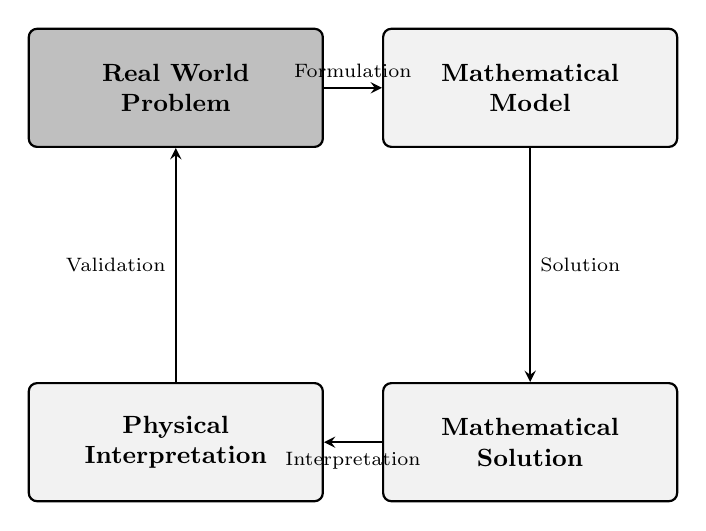
\begin{tikzpicture}[
        node distance=4.5cm, 
        auto,
        box/.style={
            draw, 
            rectangle, 
            rounded corners=3pt,
            text width=3.5cm, 
            text centered,
            minimum height=1.5cm,
            fill=gray!10,
            draw=black,
            thick,
            font=\small\bfseries
        },
        arrow/.style={
            ->,
            thick,
            >=stealth
        },
        label/.style={
            font=\scriptsize
        }
    ]
        \node (real) [box, fill=lightgray] {Real World\\Problem};
        \node (math) [box, right of=real] {Mathematical\\Model};
        \node (solution) [box, below of=math] {Mathematical\\Solution};
        \node (interpret) [box, left of=solution] {Physical\\Interpretation};
        \draw[arrow] (real) -- (math) node[midway, above, label] {Formulation};
        \draw[arrow] (math) -- (solution) node[midway, right, label] {Solution};
        \draw[arrow] (solution) -- (interpret) node[midway, below, label] {Interpretation};
        \draw[arrow] (interpret) -- (real) node[midway, left, label] {Validation};
    \end{tikzpicture}
\end{center}

\textbf{Systematic Modeling Principles:}
\begin{enumerate}
    \item Identify the relevant variables and parameters within the system
    \item Formulate assumptions to simplify the complex real-world scenario
    \item Establish the governing differential equation(s)
    \item Solve the equation using analytical or numerical methods
    \item Interpret the mathematical solution in the physical context
    \item Validate the model against experimental or observational data
    \item Refine the model iteratively to improve accuracy
\end{enumerate}

\textbf{Case Study: Population Dynamics Model}
\begin{itemize}
    \item Problem Statement: Develop a mathematical model describing temporal population variations.
    \item Fundamental Assumptions:
    \begin{itemize}
        \item Birth rate exhibits proportionality to current population size
        \item Negligible mortality, immigration, and emigration effects
        \item Unlimited environmental resources and carrying capacity
    \end{itemize}
    \item Mathematical Formulation:
    \begin{equation*}
        \frac{dP}{dt} = rP
    \end{equation*}
    where $P(t)$ represents population at time $t$ and $r$ denotes the intrinsic growth rate parameter.
\end{itemize}

\section{Enhanced Pedagogical Approach}
This course employs an improved teaching methodology that emphasizes:

\subsection{Problem-Solution Separation}
Each complex application is presented using a structured format:
\begin{itemize}
    \item \textbf{Problem Statement:} Clear presentation of the scenario and questions
    \item \textbf{Solution Framework:} Step-by-step analytical approach
    \item \textbf{Interpretation:} Physical meaning of mathematical results
\end{itemize}

\subsection{Time-Efficient Assessment Design}
Practice sessions and assessments are designed for optimal learning within allocated time:
\begin{itemize}
    \item Focused problem sets that can be completed in one hour
    \item Progressive difficulty from basic techniques to applications
    \item Emphasis on understanding over computational complexity
\end{itemize}

\subsection{Modular Learning Structure}
The course is organized into distinct modules with regular assessment:
\begin{itemize}
    \item Each module builds systematically on previous concepts
    \item Regular checkpoints ensure mastery before advancing
    \item Final integration of all course materials
\end{itemize}

\subsection{Practical Application Focus}
Real-world modeling scenarios include:
\begin{itemize}
    \item Population dynamics (exponential and logistic growth)
    \item Temperature transfer (Newton's cooling law)
    \item Chemical mixing processes
    \item Electrical circuit analysis
    \item Radioactive decay processes
\end{itemize}

% =========================================================================
% PART II: FIRST-ORDER EQUATION SOLUTION TECHNIQUES (Sessions 2-4)
% =========================================================================
\chapter{Linear Equations with Variable Coefficients and Separable Equations}
\label{chap:session_2}

This chapter covers the fundamental solution techniques for first-order differential equations.

\section{Linear Equations with Variable Coefficients}
A \textbf{first-order linear differential equation} can be written in the standard form:
\begin{equation*}
    \frac{dy}{dx} + P(x)y = Q(x)
\end{equation*}
where $P(x)$ and $Q(x)$ are continuous functions of $x$.

Key characteristics of this type of equation include:
\begin{itemize}
    \item The dependent variable $y$ and its derivative $\frac{dy}{dx}$ appear only to the first power.
    \item There are no products of $y$ and its derivatives (e.g., $y \cdot \frac{dy}{dx}$ or $(\frac{dy}{dx})^2$).
    \item The coefficients $P(x)$ and $Q(x)$ can be functions of the independent variable $x$.
\end{itemize}

\section{Method of Solution: Integrating Factor}
To solve the linear differential equation given above, we employ the method of the integrating factor.

\textbf{Step 1: Calculate the Integrating Factor}
The integrating factor, denoted by $\mu(x)$, is defined as:
\begin{equation*}
    \mu(x) = e^{\int P(x)dx}
\end{equation*}

\textbf{Step 2: Multiply by the Integrating Factor}
Multiply the entire standard differential equation by $\mu(x)$:
\begin{equation*}
    \mu(x)\frac{dy}{dx} + \mu(x)P(x)y = \mu(x)Q(x)
\end{equation*}
The left side becomes the derivative of the product $\mu(x)y$ with respect to $x$:
\begin{equation*}
    \frac{d}{dx}[\mu(x)y] = \mu(x)Q(x)
\end{equation*}

\textbf{Step 3: Integrate Both Sides}
Integrate both sides:
\begin{equation*}
    \mu(x)y = \int \mu(x)Q(x)dx + C
\end{equation*}
where $C$ is the constant of integration.

\textbf{Step 4: Solve for $y(x)$}
\begin{equation*}
    y(x) = \frac{1}{\mu(x)} \left( \int \mu(x)Q(x)dx + C \right)
\end{equation*}
This is the general solution to the first-order linear differential equation.

\section{Example: Solving a Linear Differential Equation}
Consider the differential equation:
\begin{equation*}
    x\frac{dy}{dx} - 2y = x^2 \quad \text{for } x > 0
\end{equation*}

\textbf{1. Standard Form:}
Divide by $x$:
\begin{equation*}
    \frac{dy}{dx} - \frac{2}{x}y = x
\end{equation*}
$P(x) = -\frac{2}{x}$, $Q(x) = x$.

\textbf{2. Integrating Factor $\mu(x)$:}
\begin{equation*}
    \mu(x) = e^{\int -\frac{2}{x}dx} = x^{-2}
\end{equation*}

\textbf{3. Multiply by $\mu(x)$ and Integrate:}
\begin{equation*}
    \frac{d}{dx}\left[\frac{1}{x^2}y\right] = \frac{1}{x}
\end{equation*}
Integrate:
\begin{equation*}
    \frac{1}{x^2}y = \ln x + C
\end{equation*}

\textbf{4. Solve for $y(x)$:}
\begin{equation*}
    y(x) = x^2(\ln x + C)
\end{equation*}

\section{Separable Equations}
A first-order differential equation is called \textbf{separable} if it can be written in a form where all terms involving the independent variable $x$ (and $dx$) can be moved to one side, and all terms involving the dependent variable $y$ (and $dy$) to the other.

Standard forms:
\begin{equation*}
    M(x)dx + N(y)dy = 0
\end{equation*}
or
\begin{equation*}
    \frac{dy}{dx} = f(x)g(y)
\end{equation*}

\textbf{Method of Solution: Separation and Integration}

\textbf{Step 1: Separate Variables}
\begin{equation*}
    \frac{1}{g(y)}dy = f(x)dx
\end{equation*}

\textbf{Step 2: Integrate Both Sides}
\begin{equation*}
    \int \frac{1}{g(y)}dy = \int f(x)dx + C
\end{equation*}

\textbf{Step 3: Solve for $y(x)$ (if possible)}
The result is often an implicit solution relating $x$ and $y$. If possible, solve explicitly for $y(x)$.

\section{Example: Solving a Separable Differential Equation}
Consider the differential equation:
\begin{equation*}
    \frac{dy}{dx} = \frac{x^2}{y^2}
\end{equation*}

\textbf{1. Separate Variables:}
\begin{equation*}
    y^2 dy = x^2 dx
\end{equation*}

\textbf{2. Integrate Both Sides:}
\begin{equation*}
    \int y^2 dy = \int x^2 dx
\end{equation*}
\begin{equation*}
    \frac{y^3}{3} = \frac{x^3}{3} + C_1
\end{equation*}

\textbf{3. Solve for $y(x)$:}
\begin{equation*}
    y^3 = x^3 + C
\end{equation*}
\begin{equation*}
    y(x) = \sqrt[3]{x^3 + C}
\end{equation*}
This is the general solution to the given separable differential equation.

\chapter{Modeling with First-Order Equations}
\label{chap:session_3}

This chapter covers the application of first-order differential equations to real-world modeling scenarios. We explore various physical, biological, and engineering applications through a systematic problem-solution approach.

\section{Exponential Growth Models}

\subsection{Population Growth Problem}
\textbf{Problem Statement:}
A bacteria culture has an initial population of 1000. After 2 hours, the population has grown to 1500. Assuming exponential growth:
\begin{enumerate}
    \item Find the growth rate constant.
    \item Write the population function $P(t)$.
    \item Predict the population after 5 hours.
    \item When will the population reach 10,000?
\end{enumerate}

\textbf{Solution:}
\textit{Step 1: Set up the differential equation}
For exponential growth: $\frac{dP}{dt} = kP$, where $k$ is the growth rate constant.

\textit{Step 2: Solve the differential equation}
This separable equation gives us: $P(t) = P_0 e^{kt}$

\textit{Step 3: Apply initial conditions}
Given $P(0) = 1000$, so $P_0 = 1000$.
Given $P(2) = 1500$:
\begin{align*}
1500 &= 1000e^{2k} \\
1.5 &= e^{2k} \\
k &= \frac{\ln(1.5)}{2} \approx 0.203
\end{align*}

\textit{Step 4: Complete solutions}
\begin{enumerate}
    \item Growth rate: $k \approx 0.203$ hour$^{-1}$
    \item Population function: $P(t) = 1000e^{0.203t}$
    \item After 5 hours: $P(5) = 1000e^{0.203 \times 5} \approx 2756$
    \item Time to reach 10,000: $t = \frac{\ln(10)}{0.203} \approx 11.3$ hours
\end{enumerate}

\section{Logistic Growth Models}

\subsection{Limited Population Growth Problem}
\textbf{Problem Statement:}
A population grows according to the logistic model with carrying capacity $K = 5000$ and growth rate $r = 0.1$. If the initial population is 500:
\begin{enumerate}
    \item Write the logistic differential equation.
    \item Solve for the population function $P(t)$.
    \item Find the population after 10 years.
    \item When does the population reach 90\% of carrying capacity?
\end{enumerate}

\textbf{Solution:}
\textit{Step 1: Logistic differential equation}
$\frac{dP}{dt} = rP\left(1-\frac{P}{K}\right) = 0.1P\left(1-\frac{P}{5000}\right)$

\textit{Step 2: Solve using separation of variables}
The solution to the logistic equation is:
$$P(t) = \frac{K}{1 + Ae^{-rt}}$$
where $A = \frac{K-P_0}{P_0}$

\textit{Step 3: Apply initial conditions}
With $P_0 = 500$, $K = 5000$, $r = 0.1$:
$$A = \frac{5000-500}{500} = 9$$

Therefore: $P(t) = \frac{5000}{1 + 9e^{-0.1t}}$

\textit{Step 4: Complete solutions}
\begin{enumerate}
    \item Logistic DE: $\frac{dP}{dt} = 0.1P\left(1-\frac{P}{5000}\right)$
    \item Population function: $P(t) = \frac{5000}{1 + 9e^{-0.1t}}$
    \item After 10 years: $P(10) = \frac{5000}{1 + 9e^{-1}} \approx 1839$
    \item For 90\% capacity (4500): $t = \frac{\ln(81)}{0.1} \approx 43.9$ years
\end{enumerate}

\section{Newton's Law of Cooling}

\subsection{Temperature Cooling Problem}
\textbf{Problem Statement:}
A cup of coffee at 90°C is placed in a room at 20°C. After 5 minutes, the temperature drops to 70°C. Using Newton's law of cooling:
\begin{enumerate}
    \item Find the cooling constant.
    \item Write the temperature function $T(t)$.
    \item When will the coffee reach 30°C?
\end{enumerate}

\textbf{Solution:}
\textit{Step 1: Newton's law of cooling}
$\frac{dT}{dt} = -k(T - T_{\text{ambient}})$, where $T_{\text{ambient}} = 20°\text{C}$

\textit{Step 2: Solve the differential equation}
$\frac{dT}{dt} = -k(T - 20)$
Solution: $T(t) = 20 + Ce^{-kt}$

\textit{Step 3: Apply initial conditions}
$T(0) = 90°\text{C}$ $\Rightarrow C = 70$
$T(5) = 70°\text{C}$ $\Rightarrow 70 = 20 + 70e^{-5k}$
$50 = 70e^{-5k} \Rightarrow k = \frac{\ln(7/5)}{5} \approx 0.067$

\textit{Step 4: Complete solutions}
\begin{enumerate}
    \item Cooling constant: $k \approx 0.067$ min$^{-1}$
    \item Temperature function: $T(t) = 20 + 70e^{-0.067t}$
    \item Time to reach 30°C: $t = \frac{\ln(7)}{0.067} \approx 29.0$ minutes
\end{enumerate}

\section{Mixing Problems}

\subsection{Tank Mixing Problem}
\textbf{Problem Statement:}
A tank contains 100L of pure water. Salt water with concentration 0.5 kg/L flows in at 4 L/min. The mixture flows out at the same rate, keeping the volume constant:
\begin{enumerate}
    \item Set up the differential equation for salt amount $A(t)$.
    \item Solve for $A(t)$.
    \item Find the salt amount after 30 minutes.
\end{enumerate}

\textbf{Solution:}
\textit{Step 1: Set up the differential equation}
Rate of change = Rate in - Rate out
$\frac{dA}{dt} = (0.5)(4) - \frac{A(t)}{100}(4) = 2 - \frac{A}{25}$

\textit{Step 2: Solve the linear equation}
$\frac{dA}{dt} + \frac{A}{25} = 2$
Integrating factor: $\mu = e^{t/25}$
General solution: $A(t) = 50 + Ce^{-t/25}$

\textit{Step 3: Apply initial condition}
$A(0) = 0 \Rightarrow C = -50$
Therefore: $A(t) = 50(1 - e^{-t/25})$

\textit{Step 4: Complete solutions}
\begin{enumerate}
    \item Differential equation: $\frac{dA}{dt} = 2 - \frac{A}{25}$
    \item Salt amount function: $A(t) = 50(1 - e^{-t/25})$
    \item After 30 minutes: $A(30) = 50(1 - e^{-30/25}) \approx 35.0$ kg
\end{enumerate}

\section{RC Circuit Applications}

\subsection{RC Circuit Charging Problem}
\textbf{Problem Statement:}
An RC circuit has $R = 1000\,\Omega$ and $C = 2 \times 10^{-6}$F. A 12V battery is connected at $t = 0$:
\begin{enumerate}
    \item Write the differential equation for voltage $v_C(t)$ across the capacitor.
    \item Solve for $v_C(t)$.
    \item Find the time constant and 95\% charge time.
\end{enumerate}

\textbf{Solution:}
\textit{Step 1: Kirchhoff's voltage law}
$V_{battery} = v_R + v_C = RC\frac{dv_C}{dt} + v_C$
$12 = 1000 \times 2 \times 10^{-6} \times \frac{dv_C}{dt} + v_C$
$\frac{dv_C}{dt} + 500v_C = 6000$

\textit{Step 2: Solve the linear equation}
General solution: $v_C(t) = 12 + Ce^{-500t}$
With $v_C(0) = 0$: $C = -12$
Therefore: $v_C(t) = 12(1 - e^{-500t})$

\textit{Step 3: Complete solutions}
\begin{enumerate}
    \item Differential equation: $\frac{dv_C}{dt} + 500v_C = 6000$
    \item Voltage function: $v_C(t) = 12(1 - e^{-500t})$
    \item Time constant: $\tau = RC = 0.002$ s; 95\% charge time: $t_{95\%} = 3\tau \ln(20) \approx 0.018$ s
\end{enumerate}

\chapter{Problem-Solving Workshop}
\label{chap:session_4}

This chapter provides a structured practice session focusing on first-order differential equations. The problems are designed to be completed within a one-hour timeframe, emphasizing practical application and solution techniques.

\section{Workshop Objectives}
By the end of this workshop, students should be able to:
\begin{itemize}
    \item Apply solution techniques for linear and separable first-order DEs to a variety of problems
    \item Develop strategies for setting up mathematical models from problem descriptions
    \item Analyze and interpret solutions in the context of given scenarios
    \item Enhance problem-solving skills through guided practice
\end{itemize}

\section{Warm-up Problems}

\subsection{Problem 1: Linear Equation}
Solve the initial value problem:
$$\frac{dy}{dt} + 2ty = 2te^{-t^2}, \quad y(0) = 1$$

\textbf{Solution Approach:}
\begin{itemize}
    \item Identify as a linear first-order equation
    \item Find the integrating factor: $\mu(t) = e^{\int 2t dt} = e^{t^2}$
    \item Apply the integrating factor method
    \item Use the initial condition to find the particular solution
\end{itemize}

\subsection{Problem 2: Separable Equation}
Find the general solution for:
$$\frac{dy}{dx} = \frac{x}{y}$$

\textbf{Solution Approach:}
\begin{itemize}
    \item Separate variables: $y dy = x dx$
    \item Integrate both sides: $\frac{y^2}{2} = \frac{x^2}{2} + C$
    \item Express the solution: $y^2 - x^2 = C$ (family of hyperbolas)
\end{itemize}

\section{Modeling Exercises}

\subsection{Exercise 1: Tank Mixing Problem}
A tank contains 100L of brine with 10kg of salt. Brine with 0.5 kg/L salt enters at 4 L/min and drains at the same rate.
\begin{enumerate}
    \item Set up the differential equation for salt amount $A(t)$
    \item Solve and find the salt amount after 20 minutes
\end{enumerate}

\textbf{Key Concepts:}
\begin{itemize}
    \item Rate of change = Rate in - Rate out
    \item Concentration = Amount/Volume
    \item Linear first-order equation solution
\end{itemize}

\subsection{Exercise 2: Newton's Law of Cooling}
A metal object at 80°C is placed in a 25°C room. After 10 minutes, it's 60°C.
\begin{enumerate}
    \item Write the differential equation and solve for $T(t)$
    \item Find the temperature after 30 minutes
\end{enumerate}

\textbf{Key Concepts:}
\begin{itemize}
    \item Newton's cooling law: $\frac{dT}{dt} = -k(T - T_{ambient})$
    \item Exponential decay toward ambient temperature
    \item Parameter determination from data
\end{itemize}

\section{Additional Practice Problems}

\subsection{Exercise 3: Growth with Limited Resources}
A bacteria population $P(t)$ grows according to:
$$\frac{dP}{dt} = 0.5P\left(1-\frac{P}{1000}\right)$$
Given $P(0) = 50$:
\begin{enumerate}
    \item Solve the differential equation
    \item Find the population after 5 hours
    \item What is the carrying capacity?
\end{enumerate}

\textbf{Solution Framework:}
\begin{itemize}
    \item Recognize as logistic growth model
    \item Use separation of variables or standard logistic solution
    \item Interpret parameters: growth rate and carrying capacity
\end{itemize}

\subsection{Exercise 4: Simple Decay Process}
A radioactive substance decays at a rate proportional to the amount present. If 20\% decays in 10 years:
\begin{enumerate}
    \item Set up and solve the differential equation
    \item Find the half-life of the substance
    \item How much remains after 30 years?
\end{enumerate}

\textbf{Solution Framework:}
\begin{itemize}
    \item Exponential decay model: $\frac{dN}{dt} = -\lambda N$
    \item Determine decay constant from given information
    \item Calculate half-life: $t_{1/2} = \frac{\ln(2)}{\lambda}$
\end{itemize}

\section{Key Learnings and Skills Practiced}
This workshop emphasized:
\begin{itemize}
    \item Solving linear and separable first-order differential equations
    \item Setting up mathematical models from practical scenarios
    \item Applying initial conditions and interpreting solutions
    \item Working with exponential growth, decay, and logistic models
\end{itemize}

\textbf{Focus:} Understanding the connection between problem context and mathematical models.

\section{Problem-Solving Strategy}
For successful completion of differential equation problems:
\begin{enumerate}
    \item \textbf{Identify the type} of differential equation
    \item \textbf{Choose the appropriate method} (separable, linear, etc.)
    \item \textbf{Apply the solution technique} systematically
    \item \textbf{Use initial/boundary conditions} to find particular solutions
    \item \textbf{Interpret results} in the context of the original problem
\end{enumerate}

% ============================================================================
% PART II: MODULE 2 - SECOND-ORDER DIFFERENTIAL EQUATIONS (Sessions 5-7)
% ============================================================================
\part{Second-Order Differential Equations}
\label{part:second_order_de}

\chapter{Introduction to Oscillations and Fundamental Solutions}
\label{chap:session_5}
% Session 5 content

\textit{This chapter will cover:}
\begin{itemize}
    \item Introduction to oscillatory motion
    \item Linear differential operators
    \item Fundamental solutions of homogeneous equations
    \item Characteristic equations and their roots
    \item Physical interpretation of oscillatory solutions
\end{itemize}

\chapter{Homogeneous and Non-Homogeneous Equations}
\label{chap:session_6}
% Session 6 content

\textit{This chapter will cover:}
\begin{itemize}
    \item Homogeneous linear equations with constant coefficients
    \item Complex auxiliary equations and complex roots
    \item Superposition principle
    \item Non-homogeneous equations and particular solutions
    \item Method of undetermined coefficients
\end{itemize}

\chapter{Applied Mathematical Modeling}
\label{chap:session_7}
% Session 7 content (Practice)

\textit{This chapter will include:}
\begin{itemize}
    \item Vibrations and oscillatory motion problems
    \item Method of undetermined coefficients
    \item Variation of parameters method
    \item Practical applications and examples
    \item Problem-solving techniques
\end{itemize}

% ============================================================================
% PART III: MODULE 3 - POWER SERIES SOLUTIONS AND SPECIAL FUNCTIONS (Sessions 8-10)
% ============================================================================
\part{Power Series Solutions and Special Functions}
\label{part:power_series_special_functions}

\chapter{Power Series and Taylor Series Solutions}
\label{chap:session_8}
% Session 8 content

\textit{This chapter will cover:}
\begin{itemize}
    \item Power series and analytic functions
    \item Taylor series solutions to differential equations
    \item Solutions in power series of linear differential equations
    \item Convergence and radius of convergence
    \item Applications to physics and engineering
\end{itemize}

\chapter{Cauchy-Euler Equations and Frobenius Method}
\label{chap:session_9}
% Session 9 content

\textit{This chapter will cover:}
\begin{itemize}
    \item Cauchy-Euler equations
    \item Classification of singular points
    \item Frobenius method for series solutions
    \item Orthogonal polynomials
    \item Special functions (Bessel, Legendre, etc.)
\end{itemize}

\chapter{Applications of Special Functions}
\label{chap:session_10}
% Session 10 content (Practice)

\textit{This chapter will include:}
\begin{itemize}
    \item Special functions applications in physics
    \item Series solution techniques
    \item Obtaining linearly independent solutions
    \item Boundary value problems
    \item Practical problem-solving
\end{itemize}

% ============================================================================
% PART IV: MODULE 4 - LAPLACE TRANSFORM METHODS (Sessions 11-13)
% ============================================================================
\part{Laplace Transform Methods}
\label{part:laplace_transforms}

\chapter{Definition and Properties of Laplace Transforms}
\label{chap:session_11}
% Session 11 content

\textit{This chapter will cover:}
\begin{itemize}
    \item Definition of the Laplace transform
    \item Properties and basic transforms
    \item Solution of initial value problems
    \item Transform of derivatives and integrals
    \item Inverse Laplace transforms
\end{itemize}

\chapter{Convolution and Step Functions}
\label{chap:session_12}
% Session 12 content

\textit{This chapter will cover:}
\begin{itemize}
    \item Convolution theorem and Abel problem
    \item Unit step function (Heaviside function)
    \item Impulse function (Dirac delta)
    \item Applications to engineering problems
    \item Transfer functions
\end{itemize}

\chapter{Transform Method Applications}
\label{chap:session_13}
% Session 13 content (Practice)

\textit{This chapter will include:}
\begin{itemize}
    \item Complex problem-solving using Laplace transforms
    \item Systems of differential equations
    \item Engineering applications
    \item Circuit analysis problems
    \item Mechanical vibration problems
\end{itemize}

% ============================================================================
% PART V: MODULE 5 - NON-LINEAR DIFFERENTIAL EQUATIONS (Sessions 14-16)
% ============================================================================
\part{Non-Linear Differential Equations}
\label{part:nonlinear_de}

\chapter{Autonomous Systems and Phase Portraits}
\label{chap:session_14}
% Session 14 content

\textit{This chapter will cover:}
\begin{itemize}
    \item Autonomous systems of differential equations
    \item Critical points and equilibrium solutions
    \item Stability analysis techniques
    \item Phase portraits for linear systems
    \item Classification of critical points
\end{itemize}

\chapter{Non-Homogeneous Equations and Variation of Parameters}
\label{chap:session_15}
% Session 15 content

\textit{This chapter will cover:}
\begin{itemize}
    \item Non-homogeneous linear equations
    \item Method of undetermined coefficients revisited
    \item Variation of parameters method
    \item Applications to mechanical systems
    \item Applications to electrical circuits
\end{itemize}

\chapter{Phase Portrait Construction and Applications}
\label{chap:session_16}
% Session 16 content (Practice)

\textit{This chapter will include:}
\begin{itemize}
    \item Phase portrait construction techniques
    \item Stability analysis problems
    \item Non-linear system modeling
    \item Predator-prey models
    \item Engineering applications
\end{itemize}

% ============================================================================
% PART VI: MODULE 6 - PARTIAL DIFFERENTIAL EQUATIONS (Sessions 17-19)
% ============================================================================
\part{Partial Differential Equations}
\label{part:partial_de}

\chapter{Separation of Variables and Sturm-Liouville Problems}
\label{chap:session_17}
% Session 17 content

\textit{This chapter will cover:}
\begin{itemize}
    \item Variable separation method for PDEs
    \item Sturm-Liouville boundary value problems
    \item Eigenvalues and eigenfunctions
    \item Orthogonality of eigenfunctions
    \item Applications to physics problems
\end{itemize}

\chapter{Heat, Wave, and Laplace Equations}
\label{chap:session_18}
% Session 18 content

\textit{This chapter will cover:}
\begin{itemize}
    \item The heat equation (diffusion equation)
    \item The wave equation
    \item Laplace's equation (potential theory)
    \item Boundary and initial conditions
    \item Physical interpretation of solutions
\end{itemize}

\chapter{PDE Solution Methods and Applications}
\label{chap:session_19}
% Session 19 content (Practice)

\textit{This chapter will include:}
\begin{itemize}
    \item Advanced PDE solution techniques
    \item Boundary value problems in engineering
    \item Laplace transform methods for PDEs
    \item Fourier series applications
    \item Practical problem-solving
\end{itemize}

% ============================================================================
% COMPREHENSIVE REVIEW (Session 20)
% ============================================================================

\chapter{Comprehensive Review and Integration}
\label{chap:session_20}
% Session 20 content

\textit{This chapter will include:}
\begin{itemize}
    \item Integration of all course topics
    \item Key concepts synthesis
    \item Problem-solving strategies overview
    \item Connections between different DE types
    \item Mathematical modeling competency review
\end{itemize}

\appendix
\chapter{Assessment Framework (Conceptual)}
\label{app:assessment}
While this book serves as a textual resource, the updated course assessment framework is structured as:

\section{Comprehensive Assessment Structure}
\begin{itemize}
    \item \textbf{90\% Written Assessments at End of Each Module (15\% each)}
    \begin{itemize}
        \item Six module assessments administered after modules 1-6
        \item Emphasizes conceptual understanding and practical application
        \item Each assessment covers module-specific content and skills
        \item Designed for completion within allocated session time
    \end{itemize}

    \item \textbf{10\% Final Comprehensive Assessment}
    \begin{itemize}
        \item Session 20 comprehensive evaluation
        \item Synthesizes knowledge across all course modules
        \item Integrates concepts from all six thematic modules
        \item Tests application of differential equations to complex scenarios
    \end{itemize}
\end{itemize}

\section{Assessment Philosophy}
This updated framework emphasizes:
\begin{itemize}
    \item \textbf{Modular Learning:} Regular assessment after each thematic unit
    \item \textbf{Practical Application:} Focus on problem-solving skills
    \item \textbf{Conceptual Mastery:} Understanding over memorization
    \item \textbf{Progressive Difficulty:} Building complexity throughout the course
    \item \textbf{Time Efficiency:} Assessments designed for one-hour completion
\end{itemize}

For self-study, readers are encouraged to work through examples and exercises provided in each chapter, paying particular attention to the problem-solving methodologies and modeling techniques presented.

\chapter{Recommended Texts and Further Reading}
\label{app:texts}
\textbf{Primary Text (basis for much of this material):}
\begin{itemize}
    \item Nagle, R. Kent, Saff, Edward B., Snider, Arthur David. \textit{Fundamentals of Differential Equations and Boundary Value Problems}, 9th ed. Pearson, 2018. (Updated from original reference)
\end{itemize}

\textbf{Supplementary References:}
\begin{itemize}
    \item Simmons, George F. \textit{Differential Equations with Applications and Historical Notes}, 3rd ed. CRC Press, 2017.
    \item Boyce, William E., DiPrima, Richard C., Meade, Douglas B. \textit{Elementary Differential Equations and Boundary Value Problems}, 11th ed. Wiley, 2017.
    \item Zill, Dennis G. \textit{A First Course in Differential Equations with Modeling Applications}, 11th ed. Cengage Learning, 2018.
\end{itemize}

\backmatter % For bibliography, index, etc.
% \bibliography{references} % If you have a .bib file
% \bibliographystyle{plain}

% Placeholder for a simple bibliography if not using BibTeX
\begin{thebibliography}{9}
    \bibitem{nagle2018} Nagle, R. K., Saff, E. B., \& Snider, A. D. (2018). \textit{Fundamentals of Differential Equations and Boundary Value Problems} (9th ed.). Pearson.
    \bibitem{simmons2017} Simmons, G. F. (2017). \textit{Differential Equations with Applications and Historical Notes} (3rd ed.). CRC Press.
    \bibitem{boyce2017} Boyce, W. E., DiPrima, R. C., \& Meade, D. B. (2017). \textit{Elementary Differential Equations and Boundary Value Problems} (11th ed.). Wiley.
    \bibitem{zill2018} Zill, D. G. (2018). \textit{A First Course in Differential Equations with Modeling Applications} (11th ed.). Cengage Learning.
\end{thebibliography}

\end{document}
